\section{Policy-compliant Resiliency}
Datacenter networks are highly prone to failures~\cite{datacenterfailures}, 
and it is crucial to provide certain guarantees during failure
scenarios. For example, if the operator wants to guarantee
reachability amongst endpoints, the controller only has to find an active
path in the network to re-establish reachability. 
However, upon the failure of a link, {\em reactively} synthesizing a new configuration which satisfies
all input policies can be prohibitively expensive.
Thus, we propose 
\emph{policy-compliant resiliency} to tackle network failures
by \emph{proactively} synthesizing resilient data planes that, even in the event
of a bounded number of link failures, do not violate input policies. This eliminates the 
need to resynthesize the forwarding
configuration for every network failure event.

In this section, we describe the transformation of input 
policies to provide $t-resilience$~\cite{plinko}, i.e in the event of upto $t$
arbitrary link failures, the synthesized data plane still has a path
for each packet class  satisfying all policies. This is achieved
by synthesizing backup paths satisfying input policies.
We only consider reachability, waypoint,
and isolation policies in the input. 
Global policies like capacity policies
and traffic engineering pose a difficulty in synthesis. For example,
consider a packet class $pc$ with a traffic rate of $T(pc)$. By considering
the backup paths with the same traffic characteristics for synthesis, 
the total traffic 
accounted for $pc$ would be $c\times T(pc)$ (for some constant $c$), leading
to under-provisioning of resources. Presently, \name's resilience
transformation has no provisions to avoid or minimize 
the under-provisioning of resources which affect capacity policies
and traffic engineering objectives. 
%all backup paths in consideration, while all backup paths will not 
%exist together in the network (backup paths will be deployed during
%a failure event).
%\loris{don't understand previous sentence} \kausik{Have to think!}

Given the physical topology $T=(S,L)$, a link-failure
scenario $\theta$ is defined as a set of failed links $\theta = \{l_1, l_2 \ldots ... l_n\}$,
such that $\forall i.\ l_i \in L$.
% For $t-resilience$, we need to
%consider synthesis under any set of $t$ or less arbitrary link failures.
%\begin{mydef}
	We define $\Theta(t)$ as the set of all failure scenarios where no more than $t$
	arbitrary links fail, i.e $\Theta(t) = \{ \ \theta \ \ | \ \ |\theta| \leq t\}$.
%\end{mydef}
%We define the projected topology $T^{\theta} = (S, L - \theta)$ as the active 
%physical topology under the failure scenario $\theta$. 	For each class $pc$,
%we construct a data plane graph $\xi = (S, L_{pc})$ for packet class $pc$ from the set
%of paths obtained from the synthesis algorithm. $\xi$
%for class $pc$ over a projected topology $T^\theta$ 
%is resilient if the graph $(S, L_{pc} - \theta)$ has a path from $src$ to $dst$ 
%for the packet class. 
Given a packet class $pc$,
let $\xi = (S, L_{pc})$ be the induced data plane graph obtained
by taking all the links for class $pc$ returned by the synthesis algorithm. For a failure scenario
$\theta$, the active data plane $\xi_\theta = (S, L_{pc} \setminus \theta)$ represents
all the links used by $\xi$ which are unaffected by the failure scenario. A data
plane $\xi$ is {\em resilient} to $\theta$ if it contains a path from the source to 
destination for the packet class in the active data plane $\xi_\theta$.
\begin{mydef}[Resilience]
	A data plane $\xi = (S, L_{pc})$ for class $pc$ is $t-resilient$ if $\xi$ is 
	resilient to all $\theta \in \Theta(t)$.
\end{mydef}
\begin{mydef}[Policy-compliance]
	A data plane $\xi = (S, L_{pc})$ for class $pc$ is policy-complaint if under
	any failure scenario $\theta \in \Theta(t)$, any path for $pc$ in 
	$\xi_\theta=(S, L_{pc} \setminus \theta)$ satisfies the input policies. 
\end{mydef}
\begin{algorithm}[h]
	\begin{footnotesize}
		\caption{Resilience Transformation}
		\label{restransform}
		\begin{algorithmic}[1]
			\State{[Input] $PC$: Packet classes (Reachability/Waypoint policies)}
			\State{[Input] $I$: Isolation policies (Traffic and Link types)}
			\State{[Input] $t$: Maximum number of arbitrary link failures}
			\State{[Output] $PC^R, I^R$: Transformed set of policies such that the synthesized data
				plane is $t-resilient$}
			\vspace*{0.25cm}
			\State{$PC^R, I^R \leftarrow \emptyset$}
			\For{$pc:\{src_{pc},dst_{pc},W_{pc}\} \in PC$} 
			\State{// Create $t+1$ edge-disjoint paths of $pc$}
			\State{$\hat{pc} = \{rc_1, rc_2, \ldots rc_{t+1}$\} s.t $\forall m. \ rc_m: \{src_{pc},dst_{pc},W_{pc}\}$} \label{lst:line:respc}
			\State{$PC^R = PC^R \cup \hat{pc}$} 
			\State{$I_{pc} = \{rc_m <> rc_n\ |\ \forall m,n \leq t+1 \wedge m < n\}$}  \label{lst:line:respcisolate}
			\State{$I^R = I^R \cup I_{pc}$} \label{lst:line:respcend}
			\EndFor
			\For{$i: pc_m <op> pc_n \in I$} 
			\State{$\hat{i} = \{ rc_1 <op> rc_2\ | \ \forall rc_1 \in \hat{pc_m}, \forall rc_2 \in \hat{pc_n} \}$} \label{lst:line:respolicy}
			\State{$I^R = I^R \cup \hat{i} $}
			\EndFor \\
			\Return{$PC^R, I^R$}
		\end{algorithmic}
	\end{footnotesize}
\end{algorithm}

 We now show how \Name can be modified to provide $t-resilience$.
Intuitively, this  is done by modifying the input policies so that  multiple disjoint paths satisfying the original
policies are synthesized for each packet class.
\noindent The transformation of input policies $(PC, I) \xRightarrow{res} (PC^R, I^R)$
to provide $t-resilience$ to the packet classes is described in \Cref{restransform}. 
For $t-resilience$, a packet class $pc$ needs atleast $t+1$ edge-disjoint paths from
source to destination. For this, we create $t+1$ new packet classes ($\hat{pc}$ in line~\ref{lst:line:respc})
and use link-isolation policies amongst all pairs in $\hat{pc}$ (line \ref{lst:line:respcisolate})
to create $t+1$ edge-disjoint paths for $pc$.
The synthesized data plane $\hat{\xi} = (S, L_{pc})$ for class $pc$ is constructed from the 
paths in the resilient packet class set $\hat{pc} = \{rc_1,\ldots,rc_{t+1}\}$
i.e $L_{pc} = \sum\limits_{rc \in \hat{pc}} L_{rc}$.  
Each path of $\hat{pc}$ satisfies the reachability/waypoint policy, 
and any arbitrary $t$ link failure scenario cannot affect all $t+1$ paths of $\hat{pc}$.

However, the resilient paths need to satisfy the input isolation policies with other 
packet classes (which themselves have $t+1$ paths for resilience). Thus, for a 
given policy $pc_1 || ~pc_2$, we add isolation policies to every pair of 
classes of $\hat{pc_1}$ and $\hat{pc_2}$ (line \ref{lst:line:respolicy}). This ensures that any path 
chosen in the data planes of $pc_1$ and $pc_2$ will be isolated from one 
another, thus providing policy-compliance under any arbitrary $t-link$ failure
scenario. \Cref{fig:restransform}(a) demonstrates an example transformation for providing $1-resilience$. 
\begin{theorem}[Soundness]
Given input policies $(PC, I)$, 
the data plane $\hat{\xi}_{pc}$ for every packet class $pc \in PC$
 synthesized from
transformed policies $(PC^R, I^R)$  is $t-resilient$ 
	and policy-compliant. 
\end{theorem}
\iffull
\begin{proof}
		Assume, $\exists pc$ such that the data plane $\hat{\xi} = (S, L_{pc})$
		is not $t-resilient$. 
		Therefore, there exists a failure scenario $\theta$ such that $|\theta| \leq t$ 
		and $\hat{\xi}_\theta = (S, L_{pc} \setminus \theta)$ 
		is not resilient, i.e there is no path from the source to destination. 
		Thus, $\theta$ disabled all the paths of $\hat{pc}$. \\
		However, the paths are
		edge-disjoint as each class in $\hat{pc}$ has a link-isolation policy with each 
		other. Thus, $t$ link failures cannot affect $t+1$ 
		edge-disjoint paths of $\hat{pc}$. Thus, $\theta$ disabling all paths of
		$\hat{pc}$ is a contradiction. \\
		Let us consider policy-compliance. Given a failure scenario $\theta \in \Theta(t)$, each data plane $\xi$ of class $pc$ has an active path. Consider a isolation policy in $I$: $pc_1 || \ pc_2$. In line~\ref{lst:line:respolicy} of \Cref{restransform}, each class of $\hat{pc_1}$ will be isolated to
		each class of $\hat{pc_2}$, thus any path of the data planes of $pc_1$ and
		$pc_2$ will satisfy the input policy $pc_1 || \ pc_2$. Hence, the data planes 
		are policy-compliant. 
	\end{proof}
	\fi
\noindent If there are no isolation policies in the input, the resilience transformation in lines 
\ref{lst:line:respc}-\ref{lst:line:respcend} of \Cref{restransform} is complete.
\begin{theorem}[Completeness]
%\loris{What is the input? You should say.
%Given .... such that ...., the synthesized data plane... is....if and only if...}
Given input policies $(PC,I)$ such that $I=\emptyset$,
the synthesized data plane $\xi$ for a packet class $pc$  
is $t-resilient$ if and only if it 
contains $t + 1$ edge-disjoint paths from source to destination
for $pc$.
%If there are no isolation policies $I = \emptyset$, 
%	for a packet classes $pc$, the data plane \loris{what dataplane?} is $t-resilient$ only if it 
%	contains $t + 1$ edge-disjoint paths for $pc$.
\end{theorem}
\iffull
	\begin{proof}
		We have proved the soundness of the result in \Cref{resiliencesoundness}. 
		Now, let us assume the data-plane $\hat{\xi}$ for $pc$ is $t-resilient$ such 
		that less than $t+1$ instances of $pc$ are required for resilience i.e. 
		$|\hat{pc}| < t+1$. Let us consider a 
		t-link failure scenario $\theta, |\theta| = t$ where a link is picked from
		each path of $\hat{pc}$. The active data plane
		$\hat{\xi}_\theta = (S, L_{pc} \setminus \theta)$ will not contain a
		path from source to destination as all paths of $\hat{pc}$ would be disabled.  
		This is a contradiction since $\hat{\xi}$ is $t-resilient$. 
		Therefore, we need atleast $t+1$ instances of $pc$ to ensure $t-resilience$.
		
		Now let us assume there are $t+1$ paths in a $t-resilient$ $\hat{\xi}$ for $pc$,
		and not all of them are edge-disjoint. Consider two paths $\pi_1$ and $\pi_2$
		in $\hat{\xi}$ which share a link. We can choose the shared link 
		of $\pi_1$ and $\pi_2$ and $t-1$ links from the other $t-1$ paths 
		and construct a failure scenario $\theta$, $|\theta| = t$.
		The active data plane
		$\hat{\xi}_\theta = (S, L_{pc} \setminus \theta)$ will not contain a
		path from source to destination as all paths of $\hat{pc}$ would be disabled.  
		This is a contradiction since $\xi$ is $t-resilient$. Therefore,
		the $t+1$ paths of $pc$ must be edge-disjoint. 
		
		\noindent Thus, the resilience transformation is sound and complete for a  
		packet class if there are no isolation policies.
	\end{proof}
\fi
\noindent The transformation demonstrated in \Cref{restransform} is not \emph{complete}
 if the original policies contain link-isolation policies i.e if the transformed policies
 is unsatisfiable, that does not imply the non-existence of resilient data planes. 
 \Cref{fig:restransform}(b) shows a  transformation required for $1-resilience$ 
 with fewer additional link-isolation policies among different classes
 of $pc_1$ and $pc_2$. Consider a failure scenario which disables path
 of $pc_{1A}$. By virtue of the link-isolation policies, $pc_{1B}$ and
 $pc_{2A}$ will be unaffected and can be used as paths for $pc_1$ 
 and $pc_2$ respectively, and $pc_1 <> pc_2$ holds. Now suppose
 $pc_{1B}$ is affected. Similarily, $pc_{1A}$ and $pc_{2A}$ can be used as
 the paths for the original packet classes. The same scenarios hold symmetrically
 for $pc_2$, and thus the resilience transformation can be achieved without
 adding link-isolation policies amongst all the packet classes. Therefore,
 the resilience transformation proposed in \Cref{restransform} is sound but not
 complete when the input policies comprises of isolation policies. 
 
\begin{figure}
	\centering
	\subfloat[Traffic Isolation]{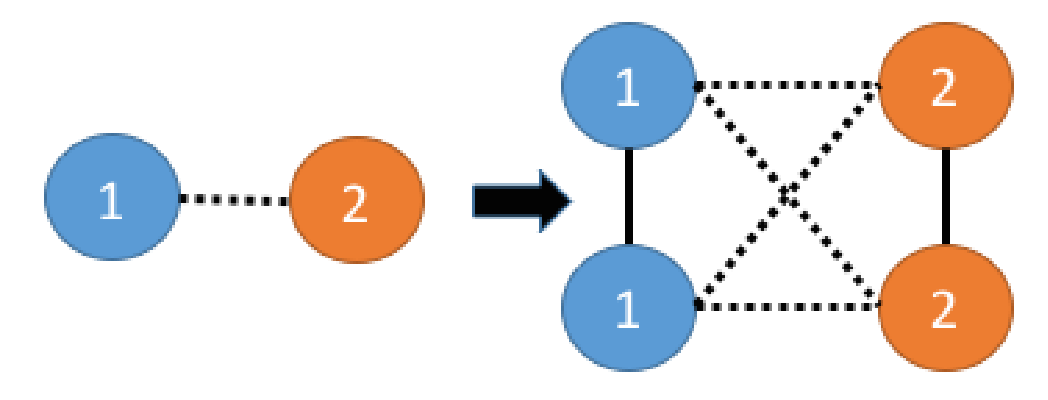
\includegraphics[width=0.5\columnwidth]{figures/resilience.eps}}
	\subfloat[Link Isolation]{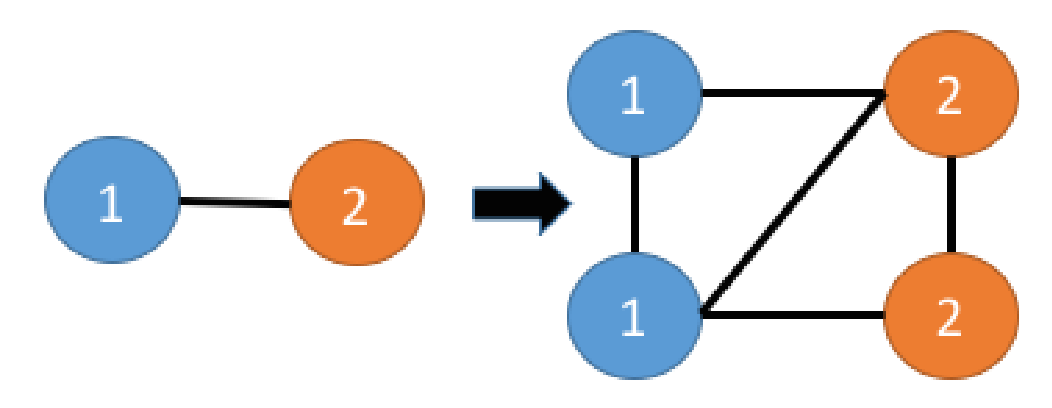
\includegraphics[width=0.5\columnwidth]{figures/resilience-cex.eps}}
	\caption{\label{fig:restransform}
		(a) Resilience Transformation for $pc_1 || \ pc_2$ for providing $1-resilience$. 
		The dotted lines represent traffic isolation policies, 
		while the solid lines represent link isolation. (b) Example of a sufficient transformation
		for 1-resilience in the case of a link-isolation policy.}
\end{figure}

We presented a sound transformation of policies to provide $t-resilience$ in
the case of reachability, waypoint and isolation policies. Future directions of 
research involve incorporating capacity constraints and traffic engineering
for synthesis of resilient data planes and devising a complete transformation for isolation.